\section{Backend}
\subsection{Grundlegender Aufbau}
\label{ch:GrundlegenderAufbau}

\subsubsection{Server}
Zur Implementierung der Geschäftslogik wird ein Webserver mit \textit{Node.js}\footnote{\url{https://nodejs.org/}} in Verbindung mit dem Framework \textit{Express}\footnote{\url{https://expressjs.com/}} verwendet.
Das Framework Express dient der Entwicklung von Webanwendungen und \acp{API}.
Diese Technologien sind weit verbreitet und vielen Teammitgliedern bereits bekannt.
Besonders letzteres spricht für die Nutzung, da keine Einarbeitungsphase notwendig ist und direkt mit der Entwicklung gestartet werden kann. 

\subsubsection{Datenbank}
Das Anbieten der \ac{API}-Endpunkte und den dazugehörigen Funktionen erfordert das serverseitige Speichern von Daten, wie die Studiengangsleiter und Dozenten.
Für die Datenhaltung wurde die Datenbank \textit{PostgreSQL}\footnote{\url{https://www.postgresql.org/}} ausgewählt, da diese relational aufgebaut ist und den Projektmitgliedern durch vorige Vorlesungen ebenfalls bereits bekannt ist.
Außerdem ist sie ziemlich verbreitet und wird von verschiedenen Frameworks unterstützt.
Ein Beispiel dafür ist \textit{Sequelize}\footnote{\url{https://sequelize.org/master/}}, ein \ac{ORM}, welches in diesem Projekt für die Anbindung der Datenbank an das Back-End verwendet wird.

\subsubsection{Architektur}
Die Architektur des Back-Ends lässt sich durch das in Abbildung \ref{fig:Schichtenmodell} dargestellte Schichtenmodell beschreiben.
Wird eine Anfrage an das Back-End gestellt, erfolgt zunächst die Authentifizierung des Benutzers.
Dazu wird geprüft, ob dieser bereits angelegt wurde und ob der mitgegebene Token dem hinterlegten Token entspricht.
Dadurch kann entschieden werden, ob die angefragte 
%mitgegebene 
Route benutzt werden darf. 

\begin{figure}[h]
	\centering 
	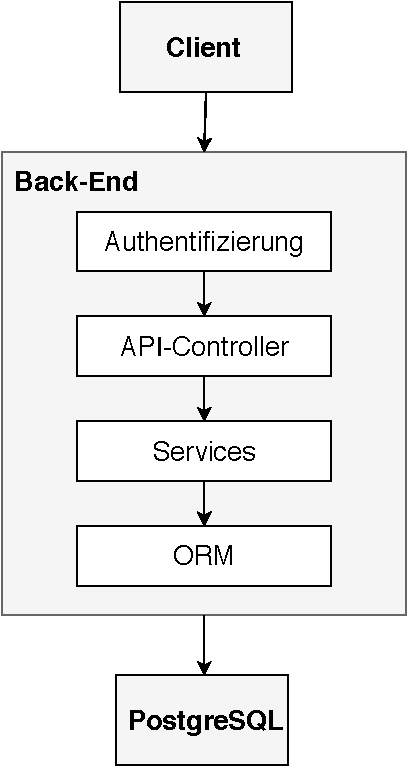
\includegraphics[width=0.4\textwidth]{img/SchichtenmodellBackend.pdf}
	\captionsetup{format=hang}
	\caption[Schichtenmodell des Back-Ends]{\label{fig:Schichtenmodell}Schichtenmodell des Back-Ends}
\end{figure}

Ist dies der Fall wird die Anfrage an die nächste Schicht weitergegeben.
Durch die API-Controller werden die Routen abgebildet.
Für jede Route gibt es einen eigenen Controller, welcher die jeweiligen \acs{HTTP}-Methoden einer Route anbietet.
Außerdem enthält diese Schicht eine Steuerlogik, welche prüft, ob die gewünschte Aktion vom Benutzer durchgeführt werden darf. 

Die Serviceschicht stellt eine Abstraktion von dem Inhalt der Datenbank bereit.
Sie definiert außerdem die \ac{ORM}-Aufrufe und stellt dadurch eine Verbindung zu dem Mapper bereit. 

Mithilfe des \ac{ORM} werden die objektorientierten Konzepte auf entsprechende relationale Konzepte abgebildet.
Auf diese Weise können Entwickler in der objektorientierten Programmiersprache bleiben, um auf die Datenbank zuzugreifen.
Dieser Zugriff erfolgt im nächsten Schritt, wenn die Daten entsprechend der gestellten Anfrage ausgelesen und an den Benutzer zurückgegeben werden. 

\subsection{API-Schnittstellen}
\subsubsection{Implementierung der Routen}
Die Routen sind an dem \ac{REST}-Paradigma orientiert, wonach nur die benötigten Informationen zurückgegeben werden.
Bei den Modulgruppen wurde jedoch davon abgewichen, da ein semantischer Zusammenhang zwischen den einzelnen Modulgruppen besteht.
Bei einem GET-Request werden immer alle Modulgruppen der angegebenen Studienrichtung zurückgegeben.
Dies vereinfacht die Programmierung im Front-End, da mit einer Anfrage an das Back-End alle Informationen zum Anzeigen eines bestimmten Modulkatalogs zurückgegeben werden.

Durch die Routen wird der Zugriff auf die vorhandenen \ac{REST}-Ressourcen gewährleistet, was unter anderem das Erstellen, Lesen, Bearbeiten und Löschen ermöglicht (CRUD-Operationen).
Für den Zugriff auf die Routen wird das \acs{HTTP}-Protokoll verwendet.
Dadurch können entsprechende Statuscodes von \acs{HTTP} verwendet werden, um eine Rückmeldung zum Erfolg oder Misserfolg einer Anfrage zu geben. 
Liegt eine fehlerhafte Anfrage vor, wird eine spezifische Fehlermeldung mit Erklärung in einem 4xx-Code an den Client gesendet.
Der \acs{HTTP}-Code 500 indiziert einen Fehler, welcher möglicherweise im Back-End liegt.


\subsubsection{Übersicht der Routen}
Die Tabellen \ref{tab:routen} und \ref{tab:adminrouten} geben eine Übersicht der zur Verfügung stehenden Routen sowie die entsprechenden \acs{HTTP}-Methoden, mit welchen auf die Routen zugegriffen werden kann. 
Tabelle \ref{tab:routen} beschreibt dabei die Routen und ihre Aktionen, die von allen Nutzern der Anwendung verwendet werden können.
Dazu zählt beispielsweise das nach Anforderung \hyperref[tab:Anforderungen]{A9} geforderte Anlegen und Löschen von Dozenten, welches mithilfe der Route \texttt{$\backslash$lecturers} durchgeführt wird. 

\begin{table}[h]
	\centering
	\renewcommand*{\arraystretch}{1.25}
	\begin{tabular}{|l|P{2cm}|P{2cm}|P{2cm}|P{2cm}|}
		\hline &&\\[-0.6em]
		\textbf{Route} & \textbf{GET} & \textbf{POST} & \textbf{PUT} & \textbf{DELETE} \\ \hline
		$\backslash$register & & x & & \\ \hline
		$\backslash$login & & x & & \\ \hline
		$\backslash$changePassword & & & x & \\ \hline
		$\backslash$academicRecords & x & x & x & x \\ \hline
		$\backslash$courses & x & x & x & x \\ \hline
		$\backslash$directorOfStudies & x & & x & \\ \hline
		$\backslash$fieldsOfStudy & x & x & x & x \\ \hline
		$\backslash$googleCalendarAPI & x & & & \\ \hline
		$\backslash$lecturerCV & x & & x & x \\ \hline
		$\backslash$lecturers & x & x & x & x \\ \hline
		$\backslash$mainFocuses & x & x & x & x \\ \hline
		$\backslash$majorSubjects & x & x & x & x \\ \hline
		$\backslash$modulecatalog & x & & & \\ \hline
		$\backslash$moduleGroups & & x & x & x \\ \hline
		$\backslash$presentations & x & x & x & x \\ \hline
		$\backslash$semesters & & x & x & x \\ \hline
		$\backslash$transferOwnership & & x & & \\ \hline
		$\backslash$usersForTransfer & x & & & \\ \hline
	\end{tabular}
	\captionsetup{format=hang}
	\caption{\label{tab:routen}Übersicht Routen \\}
\end{table}

In Tabelle \ref{tab:adminrouten} werden hingegen die Routen und Aktionen veranschaulicht, welche nur von Administratoren verwendet werden können.
Diese umfassen unter anderem das Anlegen und Auslesen von Nutzern.
Darüber hinaus kann ein Google Calendar aktualisiert sowie ein Nutzer zu einem Admin ernannt werden. 

\begin{table}[h]
	\centering
	\renewcommand*{\arraystretch}{1.25}
	\begin{tabular}{|l|P{2cm}|P{2cm}|P{2cm}|P{2cm}|}
		\hline &&\\[-0.6em]
		\textbf{Admin-Route} & \textbf{GET} & \textbf{POST} & \textbf{PUT} & \textbf{DELETE} \\ \hline
		$\backslash$createUser & & x & & \\ \hline
		$\backslash$googleCalendarAPI & & & x & \\ \hline
		$\backslash$registerKey & x & & x & \\ \hline
		$\backslash$resetPassword & & & x & \\ \hline
		$\backslash$upgradeToAdmin & & & x & \\ \hline
		$\backslash$users & x & & & \\ \hline
	\end{tabular}
	\captionsetup{format=hang}
	\caption{\label{tab:adminrouten}Übersicht Admin-Routen \\}
\end{table}

Während der Entwicklung wurden zunächst weitere Routen erstellt.
Die Entscheidungen im Laufe des Projekts haben jedoch dazu geführt, dass diese nicht mehr notwendig sind und deshalb nicht weiter entwickelt wurden.
Ein Beispiel ist die Route \texttt{$\backslash$signup}.
Diese wird nicht mehr angeboten, da eine selbstständige Registrierung nicht mehr ohne Weiteres möglich sein soll.

\subsection{Sicherheit und Zugriffskontrolle}
Da die Anwendung nur von bestimmten Personen verwendet werden soll, wird die Registrierung eingeschränkt.
Dies erfolgt über einen Registrierungsschlüssel, welcher bei einer Registrierung angegeben werden muss.
Ein solcher Schlüssel ist dem Administrator bekannt und dieser kann einen neuen Registrierungsschlüssel festlegen.
Zusätzlich besteht die Möglichkeit, dass der Administrator selbst Benutzer zum System hinzufügt. 

Des Weiteren sollen in der Anwendung nur benutzerspezifische Inhalte angezeigt werden und der Benutzer darf nur die Aktionen durchführen, zu denen er berechtigt ist.
Dafür muss ein Nutzer identifiziert werden können, weshalb eine digitale Identität erstellt wird.
Dies erfolgt durch die Registrierung mit Mail-Adresse und Passwort, entsprechend der Anforderung \hyperref[tab:Anforderungen]{A4}.

Für die Verifizierung des Passworts bei der Anmeldung eines Nutzers, muss das Passwort gespeichert werden.
Damit dieses nicht ausgelesen und für unberechtigten Zugang zu der Software genutzt werden kann, wird das Passwort als Hash-Wert gespeichert.
Die Erstellung des Hash-Werts erfolgt mithilfe der Node.js-Bibliothek \textit{bcrypt}\footnote{\url{https://www.npmjs.com/package/bcrypt}}.
Diese baut auf der kryptographische Hashfunktion bcrypt auf, welche speziell für das Hashen und Speichern von Passwörtern entwickelt wurde.
%Dieser wird mithilfe der Node.js-Bibliothek \textit{bcrypt}\footnote{\url{https://www.npmjs.com/package/bcrypt}} erstellt.
%Bcrypt ist eine kryptographische Hashfunktion speziell für Passwörter. 

Um jedoch eine häufige Verwendung des Passworts zu vermeiden wird ein \textit{JSON Web Token}\footnote{\url{https://jwt.io/}} generiert, welcher ein genormtes Access-Token darstellt.
Bei der Registrierung und Anmeldung eines Nutzers wird ein solcher Token ausgestellt, der bei anschließenden Anfragen an das Back-End mitgegeben wird.
Dieses prüft daraufhin die Korrektheit des Tokens bevor eine Aktion durchgeführt wird.
Ist der Nutzer gespeichert und der Token hinterlegt, ist dieser berechtigt Anfragen zu senden.
Außerdem wird bei jedem Aufruf der Controllern geprüft, ob eine Aktion valide ist.
Auf diese Weise wird bspw. verhindert, dass ein Studiengangsleiter die Kurse eines anderen ändern kann. 

Ähnlich wie Passwörter nicht im Klartext gespeichert werden sollten, sollte auch die Kommunikation zwischen Client und Server nicht im Klartext erfolgen.
Deshalb wird das sichere Kommunikationsprotokoll \acs{HTTPS} verwendet.
Dadurch werden die Nachrichten verschlüsselt übertragen, was insbesondere für die Übermittlung von Passwörtern und Token wichtig ist. 